\chapter{\IfLanguageName{dutch}{literatuurstudie}{Introduction}}%
\label{ch:Literatuurstudie}

\subsection{Back-ups in het kader van bedrijfscontinuïteit en disaster recovery}
Bedrijfscontinuïteit verwijst naar de aanpak en procedures dat een bedrijf gebruikt om de voortgang van zijn werkzaamheden te bewaren, zelfs in het geval van incidenten. Deze incidenten kunnen variëren van relatief kleine problemen, zoals een gebroken netwerkverbinding, tot grote natuurrampen zoals een aardbevingen. Omdat er zoveel soorten incidenten kunnen gebeuren is het moeilijk om een oplossing te vinden die ervoor zorgt dat bedrijven in alle gevallen beschermt zijn. In plaats daarvan gebruiken bedrijven een mix van strategieën en technologieën om de continuïteit van hun processen te beschermen. De 2 belangrijkste concepten voor de bedrijfscontinuïteit zijn hoge beschikbaarheid en disaster recovery. Hoge beschikbaarheid duidt op het feit dat een bedrijf zodanig is ingericht dat het kan blijven draaien, zelfs als bepaalde systemen of componenten uitvallen. Een voorbeeld hiervan zijn twee routers die zijn geconfigureerd in een actieve-passieve opstelling. In deze configuratie is één router de primaire router die al het inkomende en uitgaande verkeer verwerkt, terwijl de andere router als reserve werkt. In het geval dat de primaire router faalt door een hardwarestoringen of netwerkprobleem, dan neemt de tweede router automatisch de rol van de primaire router over, zonder dat dit merkbare impact heeft op de netwerkverbindingen van de organisatie. Hierdoor blijft de beschikbaarheid van het netwerk gegarandeerd en blijft de downtime laag \autocite{Zhu2015}. Disaster recovery (DR) is een onderdeel van bedrijfscontinuïteit dat zich specifiek richt op het herstellen van bedrijfsactiviteiten na een incident zoals een cyberaanval of ernstige verstoring. Terwijl bedrijfscontinuïteit zich richt op bredere preventieve maatregelen om de continuïteit te waarborgen, focust disaster recovery zich juist op de praktische stappen en hulpmiddelen die nodig zijn om de organisatie na een verstoring weer snel operationeel te maken. Het doel van disaster recovery is om schade zoveel mogelijk te beperken en de normale gang van zaken zo snel mogelijk te herstellen. Back-ups spelen een belangrijke rol voor de continuïteit van een bedrijf en zijn vaak de eerste stap bij het opstellen van een disaster recovery plan (DRP). Bij een optimale situatie is er na een incident geen data verloren en is alle data relatief snel terug beschikbaar. Indien een bedrijf geen back-ups heeft van de belangrijke data zal de data in het geval van een incident verloren raken. Zonder back-ups zal het ook een grotere uitdaging zijn voor het bedrijf om de normale bedrijfsactiviteiten terug uit te voeren. Een belangrijke doelstelling van een bedrijf is winst maken. In het geval van een incident waarbij de bedrijfsactiviteiten niet normaal kunnen verlopen zal deze doelstelling verhindert worden en zal er dus financieel verlies optreden. Bij specifieke bedreigingen, zoals ransomware-aanvallen spelen ransomware-resistente back-ups een cruciale rol. Door back-ups te beveiligen tegen ransomware-aanvallen kunnen bedrijven hun data herstellen zonder losgeld te betalen. Dit benadrukt het belang van back-ups die niet alleen snel toegankelijk zijn, maar ook bestand zijn tegen digitale bedreigingen \autocite{Ghazi2013}.

\subsection{Back-upmethoden en -technieken}
Back-ups zijn een belangrijk onderdeel van datamanagement en databeveiliging binnen organisaties. Back-ups zorgen voor de continuïteit van bedrijfssystemen in het geval van een incident zoals een cyberaanval. Back-ups zijn snapshots van gegevens die op een bepaald tijdstip zijn gemaakt, opgeslagen in een wereldwijd gebruikelijk formaat en gedurende een bepaalde periode van bruikbaarheid worden bijgehouden, waarbij elke volgende kopie van de gegevens onafhankelijk van de eerste wordt bewaard\autocite{Nelson2011}. Door een aparte kopie van de gegevens te bewaren, kunnen bedrijven en individuen na een incident hun systemen of bestanden herstellen naar een eerdere, veilige staat. Hierbij kunnen back-ups zowel volledige datasets als selectieve bestandstypen omvatten, afhankelijk van de strategie en de specifieke behoeften van de organisatie. Back-ups zijn een preventieve maatregel en het doel ervan is om dataverlies tegen te gaan. Dataverlies kan optreden door menselijke fouten, cyberaanvallen, en natuur- of bedrijfsrampen. Daarbij speelt beveiliging een belangrijke rol in een tijd waarin ransomware-aanvallen en datalekken frequenter voorkomen. Door back-ups versleuteld op te slaan en te beveiligen tegen ongeautoriseerde toegang, kunnen bedrijven zich beschermen tegen het verliezen van data. 
\subsubsection{Full back-ups}
\begin{figure}[h] 
    \centering
    \captionsetup{justification=centering}
    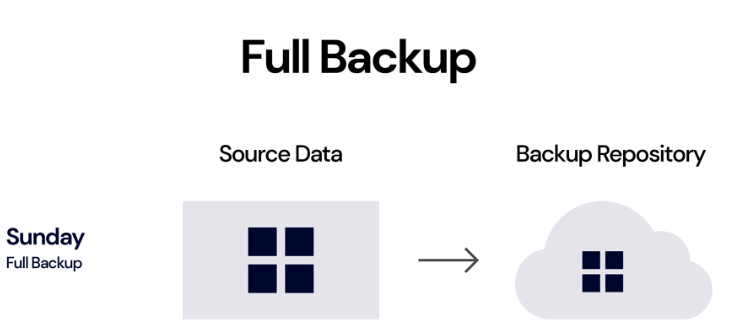
\includegraphics[width=\textwidth]{img/fullb.png}  
    \caption{Representatie van een full back-up \autocite{Rivas2022}}   
    \label{fig:fullback-up}           
\end{figure}
Een full back-up is een back-upmethode waarbij alle gegevens van een systeem op een specifiek moment volledig worden gekopieerd en opgeslagen. Dit betekent dat elk bestand zonder uitzonderingen wordt gekopieerd, zodat er een exacte kopie van de volledige dataset ontstaat \autocite{Beard2018}. Wanneer er zich een probleem voordoet, zoals het falen van een harde schijf, kan het hele bestandssysteem vanaf deze back-up volledig worden hersteld op een nieuwe schijf. Daarnaast kunnen ook individuele bestanden die verloren zijn gegaan, gemakkelijk worden teruggehaald uit de back-up. Dit soort back-up zorgt ervoor dat alle gegevens veilig zijn opgeslagen \autocite{Chervenak1998}. Full back-ups vormen vaak de basis van een back-upstrategie en worden regelmatig uitgevoerd om ervoor te zorgen dat alle gegevens volledig hersteld kunnen worden. Het concept en de implementatie van een full back-up is relatief eenvoudig omdat alle gegevens op één locatie zijn opgeslagen. Aan de andere kant is er het probleem van opslagcapaciteit. Stel bijvoorbeeld dat een bedrijf elke nacht een full back-up maakt van zijn servers naar een cloudopslagdienst, waarbij per keer 500 GB aan data wordt opgeslagen. Na een week is er al 3,5 terabyte aan gegevens in de cloud opgeslagen. Aangezien cloudproviders vaak kosten in rekening brengen op basis van gebruikte opslagcapaciteit en dataverkeer, kan dit snel leiden tot aanzienlijke maandelijkse kosten. Bedrijven met een beperkt IT-budget kunnen hierdoor in de problemen komen of worden gedwongen om strenger te selecteren welke gegevens ze precies opslaan in de back-up, omdat de opslagkosten oplopen naarmate de hoeveelheid opgeslagen data toeneemt. Daarbij kan het proces zelf ook veel tijd innemen. Dit kan voor problemen zorgen bij bedrijven waarbij de systemen aan moeten blijven. Vaak worden full back-ups gecombineerd met andere back-upmethodes. Daarnaast kost een full back-up veel tijd, wat een uitdaging kan zijn in omgevingen waar snelle gegevensbeschikbaarheid nodig is. Stel bijvoorbeeld dat een groot bedrijf tijdens kantooruren een full back-up wil maken van alle gegevens. Omdat deze back-up meerdere uren in beslag kan nemen, worden de systemen gedurende die tijd zwaar belast. Dit kan ertoe leiden dat andere processen vertraging oplopen of dat de server tijdelijk minder goed beschikbaar is voor werknemers die ook van die systemen afhankelijk zijn voor hun dagelijkse taken. Vanwege deze nadelen is het vaak beter om full back-ups aan te vullen met andere methoden \autocite{Nelson2011}.

\subsubsection{Incrementele back-up}
\begin{figure}[h] 
    \centering
    \captionsetup{justification=centering}
    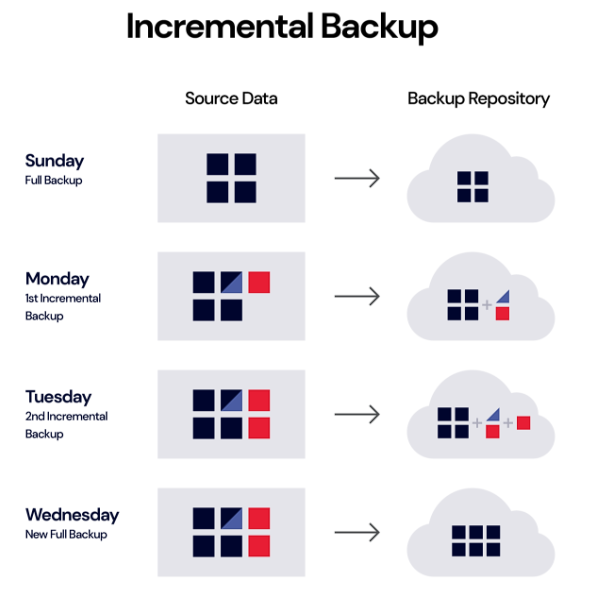
\includegraphics[width=0.5\textwidth]{img/incrementb.png}  
    \caption{Representatie van een incremental back-up \autocite{Rivas2022}}   
    \label{fig:incrback-up}           
\end{figure}

Een incrementele back-upstrategie houdt in dat na een initiële full back-up slechts de gegevens worden opgeslagen die sinds de laatste back-up zijn gewijzigd \autocite{Zhao2024}. Dit betekent dat een incrementele back-up alleen de veranderingen in de bestanden opneemt, in plaats van telkens een volledige kopie te maken van alle gegevens. Dit is vooral handig voor bedrijven die relatief vaak back-ups moeten maken, maar de opslag- en tijdskosten van een full back-up willen vermijden. Bijvoorbeeld, stel dat een bedrijf op maandag een full back-up uitvoert met al hun gegevens. Op dinsdag doet het bedrijf een incrementele back-up, waarbij enkel de wijzigingen sinds maandag worden opgeslagen. Dit gaat elke dag zo verder, elke dag wordt enkel de nieuwe of gewijzigde data opgeslagen ten opzichte van de dag ervoor. Omdat bedrijven steeds meer data beheren, biedt deze methode een efficiënte manier om opslagkosten te beperken, vooral wanneer gebruik wordt gemaakt van een cloudservice. Stel dat een bedrijf dagelijks slechts 1\% van zijn gegevens wijzigt; in plaats van elke dag een volledige kopie van bijvoorbeeld 1 TB te maken, slaat een incrementele back-up slechts de nieuwe 1\% op, wat 990 GB aan opslagruimte per dag bespaart. Dit maakt incrementele back-ups heel aantrekkelijk voor bedrijven die grote hoeveelheden data verwerken en frequente back-ups willen uitvoeren. Naast de besparing op opslagcapaciteit, zorgen incrementele back-ups voor kortere back-uptijden omdat alleen de gewijzigde bestanden worden opgeslagen. Dit betekent dat bedrijven vaker back-ups kunnen uitvoeren zonder hun systemen te vertragen. Een mediabedrijf dat met grote bestanden werkt, kan hierdoor bijvoorbeeld elk uur een incrementele back-up maken, in plaats van dagelijks een volledige back-up. Dit minimaliseert het risico op dataverlies, omdat in het geval van een storing, slechts maximaal een uur aan data verloren gaat in plaats van een hele dag. Hoewel incrementele back-ups voordelen bieden op het gebied van opslag en back-uptijden, brengen ze ook nadelen met zich mee, zoals langere hersteltijden\autocite{Chervenak1998}. Om een systeem te herstellen, heb je de laatste volledige back-up en alle volgende incrementele back-ups nodig en dit kan veel tijd kosten. Een financiële instelling die bijvoorbeeld op vrijdag een een systeemherstel moet uitvoeren, zal de volledige back-up van maandag plus alle incrementele back-ups tot en met donderdag moeten doorlopen. Dit kan relatief lang duren, wat leidt tot langere downtime, vooral in een noodsituatie waarin snelle hersteltijd van belang is. Een ander nadeel is de complexiteit van het beheer. Elke incrementele back-up hangt af van de vorige, wat betekent dat een fout in één back-up de hele herstelketen kan verstoren. Een IT-bedrijf dat dagelijks incrementele back-ups maakt, kan bijvoorbeeld problemen ondervinden als de back-up van woensdag beschadigd blijkt te zijn. Alle latere back-ups zijn afhankelijk van die ene back-up, wat het herstelproces moeilijker maakt. Dit vraagt om extra monitoring en beheer, zodat eventuele beschadigingen of herstelproblemen tijdig kunnen worden opgemerkt en opgelost.
\subsubsection{Differentiële back-ups}
 \begin{figure}[h]
    \centering
    \captionsetup{justification=centering}
    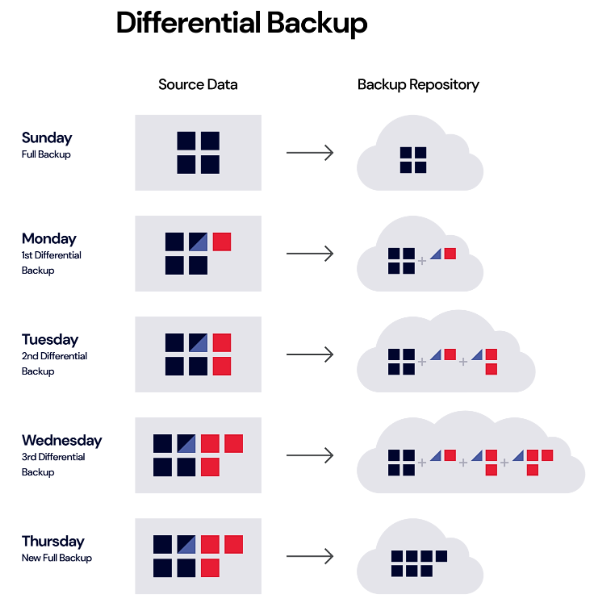
\includegraphics[width=0.5\textwidth]{img/diff.png}  
    \caption{Representatie van een differentiële back-up \autocite{Rivas2022}}   
    \label{fig:diffrback-up}           
\end{figure}
Een differentiële back-up is een soort back-up waarbij enkel de data die sinds de laatste full back-up is veranderd of toegevoegd, wordt gekopieerd. In tegenstelling tot een incrementele back-up, die enkel de veranderingen sinds de laatste back-up opslaat, wordt er bij een differentiële back-up enkel de wijzigingen opgeslagen sinds de laatste full back-up \autocite{Zhu2015}. Een differentiële back-up zal dus elke keer groter en groter worden naarmate er meer wijzigingen zijn omdat elke wijziging sinds de full back-up opgeslagen wordt. Een eerste voordeel van deze soort back-up is dat er in het geval van een recovery slechts twee back-ups nodig zijn: de laatste full back-up en de meest recente differentiële back-up. Wanneer hersteltijden belangrijk zijn zullen differentiële back-ups dus handig zijn. Bijvoorbeeld, een organisatie die dagelijks een differentiële back-up uitvoert, heeft na een week slechts de volledige back-up van de eerste dag en de laatste differentiële back-up nodig om alles te herstellen. Dit zorgt voor een relatief eenvoudig en snel herstelproces. Incrementele back-ups daarentegen slaan alleen de veranderingen op die sinds de laatste back-up zijn gemaakt van eender welke soort, of het nu een volledige of incrementele back-up is. Hierdoor zijn incrementele back-ups meestal kleiner en sneller uit te voeren dan differentiële back-ups, omdat ze alleen de allerlaatste wijzigingen bevatten. Een eerder besproken nadeel is echter dat bij herstel alle opeenvolgende back-ups nodig zijn om de data volledig terug te zetten: de laatste volledige back-up en alle incrementele back-ups tot de meest recente back-up. Dit maakt incrementele back-ups soms trager en complexer bij recovery, omdat elk back-upbestand moet worden doorlopen. Een voorbeeld om het verschil tussen incrementele back-ups en differentiële back-ups duidelijk te maken: stel dat een bedrijf aan het begin van de week een volledige back-up maakt. Bij het gebruik van een differentieel back-upschema zou elke back-up in de loop van de week groter worden, omdat elke back-up alle wijzigingen sinds die eerste dag bevat. Bij een incrementeel schema daarentegen blijft elke dagelijkse back-up klein, omdat elke nieuwe back-up alleen de nieuwste wijzigingen bevat. Als het systeem aan het einde van de week moet worden hersteld, zou met een differentieel schema enkel de full back-up en de laatste differentiële back-up nodig zijn. Bij het gebruik van incrementele-backups zijn alle back-ups van de week vereist.\autocite{Beard2018}

\subsubsection{Cloud back-ups}
Cloud back-ups zijn een populaire methode waarbij data op externe servers wordt opgeslagen, beheerd door een derde partij. In plaats van lokale fysieke opslagapparaten te gebruiken, worden de gegevens overgebracht naar een cloudomgeving, zoals die van Amazon Web Services, Microsoft Azure of Google Cloud. Cloud back-ups bieden verschillende voordelen, zoals schaalbaarheid, eenvoud in beheer en de mogelijkheid om gegevens veilig op afstand op te slaan. Voor bedrijven betekent dit dat zij geen dure fysieke hardware hoeven aan te schaffen, en de infrastructuur flexibel kunnen aanpassen aan hun behoeften. Een bedrijf dat bijvoorbeeld snel groeit, kan zijn cloudopslag uitbreiden zonder ingrijpende veranderingen aan de interne IT-omgeving. Een van de belangrijkste voordelen van cloud back-ups is toegankelijkheid. Aangezien de gegevens zich op een externe server bevinden, kan een bedrijf op elk moment en vanaf elke locatie toegang krijgen tot zijn data, zolang er een internetverbinding is. Dit kan cruciaal zijn voor organisaties met vestigingen op meerdere locaties. Stel dat een bedrijf werkt met een gedistribueerd team: de medewerkers kunnen overal ter wereld op dezelfde up-to-date back-ups vertrouwen, wat de samenwerking vergemakkelijkt en de continuïteit waarborgt, zelfs in noodsituaties. Daarnaast biedt cloudopslag een hoge mate van beveiliging, aangezien cloudproviders meestal robuuste beveiligingsprotocollen implementeren, zoals encryptie, firewalls en multi-factor authenticatie. Voor veel kleinere bedrijven betekent dit dat zij kunnen profiteren van een hoger beveiligingsniveau zonder te investeren in geavanceerde beveiligingsinfrastructuur. Stel dat een middelgroot marketingbureau zijn klantgegevens in de cloud opslaat; de back-ups zijn dan beschermd tegen onvoorziene omstandigheden, zoals fysieke schade aan hun eigen kantoren. Echter, cloud back-ups hebben ook nadelen, waaronder de afhankelijkheid van een stabiele internetverbinding. Omdat cloud back-ups vereisen dat data over het internet wordt verzonden, kunnen problemen met de internetverbinding de back-uptijd vertragen of de overdracht volledig onderbreken. Voor een organisatie die bijvoorbeeld grote hoeveelheden videobestanden moet opslaan, kan dit tijdsverlies betekenen, vooral wanneer zij gevestigd zijn op een locatie met beperkte bandbreedte. Dit kan een probleem vormen wanneer er een strikte back-upfrequentie vereist is. Een ander nadeel is de kostprijs, vooral wanneer grote hoeveelheden gegevens vaak worden geüpdatet en opgeslagen. Cloudopslagproviders rekenen doorgaans kosten voor opslagcapaciteit, maar ook voor dataverkeer en extra functies zoals geavanceerde encryptie of frequentere back-ups. Voor een bedrijf dat veel wijzigingen aanbrengt in grote databases, zoals een online retailer met dagelijks nieuwe productinformatie, kunnen de maandelijkse kosten aanzienlijk oplopen. Dit maakt het noodzakelijk om een weloverwogen keuze te maken over de frequentie en omvang van back-ups om de kosten beheersbaar te houden. Tot slot biedt de cloud niet altijd dezelfde mate van controle als on-premise oplossingen. Hoewel cloudproviders doorgaans goede service garanderen, blijft het bedrijf afhankelijk van de beschikbaarheid en het onderhoudsbeleid van de provider. Dit betekent dat, in het geval van een storing bij de cloudprovider, bedrijven geen directe toegang hebben tot hun eigen back-ups. Een juridische firma die vertrouwelijke documenten in de cloud opslaat, kan bijvoorbeeld beperkte toegang hebben tot deze gegevens als de cloudprovider technische problemen ondervindt. Dit benadrukt het belang van goed service level agreements (SLA's) en mogelijk zelfs een hybride strategie die cloudopslag combineert met een bepaalde vorm van lokale back-ups om het risico te spreiden.


\subsubsection{On-premise back-ups}
On-premise back-ups zijn back-ups die lokaal worden opgeslagen op de fysieke servers en opslagapparaten binnen de infrastructuur van een bedrijf. Deze methode houdt in dat het bedrijf zelf verantwoordelijk is voor het beheren, beveiligen en onderhouden van de back-upomgeving. Voor organisaties die volledige controle willen over hun gegevens, bieden on-premise back-ups een direct en tastbaar voordeel: de data blijft in eigen beheer, wat vooral waardevol is in sectoren waar data security en privacy van groot belang zijn, zoals de gezondheidszorg of financiële dienstverlening. Een van de grootste voordelen van on-premise back-ups is dat er geen afhankelijkheid is van een internetverbinding. Aangezien de back-up lokaal gebeurt, is de snelheid van het netwerk binnen het bedrijf bepalend voor de snelheid van het back-upproces. Voor een organisatie met een snelle interne netwerkinfrastructuur, zoals een mediabedrijf dat dagelijks grote videobestanden back-upt, kan dit het verschil maken tussen uren en minuten. Dit maakt on-premise back-ups een ideale keuze voor bedrijven die snel grote hoeveelheden data moeten opslaan zonder gehinderd te worden door internetbeperkingen. Daarnaast biedt on-premise opslag de mogelijkheid om de volledige back-up- en herstelstrategie te personaliseren en aan te passen aan de specifieke behoeften van de organisatie. Dit kan belangrijk zijn voor bedrijven die bepaalde compliance-eisen hebben of die willen experimenteren met specifieke back-uptechnieken, zoals differential of incremental back-ups. Een bedrijf in de financiële sector kan bijvoorbeeld ervoor kiezen om alle dagelijkse transacties lokaal op te slaan en de volledige back-ups wekelijks op een afgescheiden server te bewaren. Op deze manier kunnen zij hun data volledig beheren, met maatregelen die specifiek zijn afgestemd op hun eigen risico’s en beleid. Toch komen on-premise back-ups met aanzienlijke nadelen. Een belangrijke uitdaging is de hoge initiële investering in hardware en onderhoud. Bedrijven moeten investeren in servers, harde schijven, netwerkinfrastructuur en mogelijk zelfs koeling- en beveiligingssystemen. Voor een middelgroot productiebedrijf dat bijvoorbeeld zijn back-ups op eigen servers wil opslaan, kan dit een aanzienlijke uitgave betekenen. Bovendien moeten deze systemen regelmatig worden geüpdatet en vervangen, wat extra kosten en logistieke planning met zich meebrengt. Een ander nadeel van on-premise back-ups is dat ze gevoelig zijn voor fysieke risico’s zoals brand, diefstal of overstromingen. Aangezien de gegevens op locatie zijn opgeslagen, kunnen ze verloren gaan als de infrastructuur fysiek wordt beschadigd. Dit betekent dat bedrijven extra beveiligingsmaatregelen moeten nemen, zoals een secundaire back-up op een externe locatie. Stel dat een IT-bedrijf zijn servers in zijn hoofdkantoor opslaat en daar een brand uitbreekt; dan zijn zowel de primaire data als de back-up data in gevaar, tenzij er een tweede kopie offsite is opgeslagen. Dit vergroot de behoefte aan een goed doordachte noodherstelstrategie. Daarnaast vereisen on-premise back-ups specifieke IT-expertise om een goed beheerde en beveiligde omgeving te handhaven. Het interne IT-team moet in staat zijn om regelmatig back-ups uit te voeren, beveiligingsupdates bij te houden, en ervoor te zorgen dat de gegevens ten alle tijden toegankelijk en veilig zijn. Voor een kleine organisatie zonder een toegewijd IT-team kan dit een uitdaging zijn, aangezien deze taken continu onderhoud en aandacht vereisen.
\subsubsection{Offline back-ups}
Offline back-ups zijn back-ups die fysiek worden opgeslagen op opslagmedia zoals externe harde schijven, tape-drives of andere niet-aangesloten apparaten, zonder constante verbinding met het netwerk of internet. Het belangrijkste verschil met on-premise back-ups is dat offline back-ups na het maken ervan van het netwerk worden losgekoppeld, waardoor ze immuun worden voor online bedreigingen zoals ransomware of hacking. Bij on-premise back-ups blijven de gegevens meestal beschikbaar binnen de lokale netwerkomgeving van het bedrijf, terwijl offline back-ups juist fysiek worden verwijderd van elke vorm van netwerktoegang. Een van de grootste voordelen van offline back-ups is dat ze een extra laag bescherming bieden tegen cyberaanvallen. Doordat deze back-ups niet online toegankelijk zijn, kunnen kwaadwillenden er via het netwerk geen toegang toe krijgen. Dit kan een essentieel voordeel zijn voor bedrijven die met gevoelige gegevens werken, zoals een advocatenkantoor dat juridische documenten opslaat. Stel dat een ransomware-aanval het hele netwerk vergrendelt, dan blijven de offline back-ups onaangetast, omdat ze fysiek losgekoppeld zijn van het geïnfecteerde systeem. Op deze manier kunnen bedrijven hun gegevens nog steeds herstellen, zelfs in het geval van een grote cyberaanval. Offline back-ups bieden ook het voordeel van fysieke controle. Een bedrijf dat zijn offline back-ups in een kluis of beveiligde ruimte opslaat, heeft de zekerheid dat de gegevens veilig zijn tegen zowel digitale als sommige fysieke bedreigingen. Dit is bijvoorbeeld handig voor een onderzoeksorganisatie die vertrouwelijke onderzoeksgegevens heeft en ervoor wil zorgen dat alleen bevoegde personen toegang hebben. Door de back-ups fysiek op te slaan in een beveiligde ruimte kan worden bepaald wie wanneer bij de data kan. Echter, offline back-ups brengen ook enkele nadelen met zich mee. Een van de grootste uitdagingen is dat ze handmatig moeten worden bijgewerkt, wat arbeidsintensief kan zijn. Dit kan een probleem vormen voor bedrijven met zeer regelmatig veranderende gegevens. Neem een klein e-commercebedrijf dat elke dag nieuwe verkoopgegevens verzamelt en opslaat; om deze data te beschermen, zou dagelijks een offline back-up moeten worden gemaakt en fysiek worden opgeborgen. Dit proces kan tijdrovend zijn en vereist dat er een routine is om deze back-ups nauwgezet te beheren. Een ander nadeel van offline back-ups is dat ze kwetsbaar blijven voor fysieke schade, verlies of diefstal. Aangezien ze worden opgeslagen op fysieke media, zijn ze gevoelig voor gebeurtenissen zoals brand, waterschade of diefstal. Een mediabedrijf dat zijn videoprojecten op tapes opslaat, loopt bijvoorbeeld het risico dat al zijn gegevens verloren gaan als er brand uitbreekt in de opslagruimte. Het gebruik van een tweede offsite opslaglocatie kan hier een oplossing bieden, maar dat brengt extra kosten en logistiek met zich mee. Daarnaast is de toegang tot offline back-ups vaak minder flexibel en kan het herstelproces langer duren. Doordat de gegevens fysiek moeten worden aangesloten en overgezet naar een systeem, kan het tijd kosten om data te herstellen. Stel dat een productiebedrijf te maken krijgt met een systeemfout en de gegevens uit een offline back-up moet herstellen. Het proces kan langer duren dan bij een online back-up, omdat het opslagmedium fysiek moet worden aangesloten en de gegevens moeten worden overgezet naar het netwerk. Dit betekent dat offline back-ups minder geschikt zijn voor bedrijven die minimale downtime nodig hebben.

\subsection{Ransomware}
\subsection{Ransomware-resistente back-upoplossingen}
\subsubsection{Air-gapped back-ups}
\subsubsection{Immutable storage}
Immutable storage, of onveranderbare opslag, is een techniek waarbij opgeslagen gegevens na het opslaan niet kunnen worden gewijzigd of verwijderd gedurende een vooraf vastgelegde periode. Dit biedt een sterke bescherming tegen cyberaanvallen, zoals ransomware, en menselijke fouten, aangezien gegevens na het vastleggen immuun zijn voor wijzigingen. Het concept van immutable storage komt vooral van pas bij organisaties die te maken hebben met zeer gevoelige gegevens en die moeten kunnen garanderen dat hun data altijd veilig en betrouwbaar blijft. Het belangrijkste voordeel van immutable storage is dat het data beschermt tegen kwaadwillende wijzigingen. Stel bijvoorbeeld dat een financiële instelling haar financiële rapporten opslaat met immutable storage. Als een ransomware-aanval probeert om de gegevens te versleutelen of te verwijderen, zal de immutable opslag de wijziging blokkeren, zodat de originele, ongewijzigde data beschikbaar blijft. Dit biedt organisaties die werken met onvervangbare gegevens een vrijwel onaantastbare zekerheid, aangezien geen enkele vorm van digitale aanval de opgeslagen gegevens kan wijzigen of verwijderen. Immutable storage is vooral effectief als back-upoplossing. Een onderneming die regelmatig back-ups maakt in een immutable storage-omgeving, kan erop rekenen dat deze back-ups intact blijven, zelfs als het hoofdnetwerk wordt aangevallen. Denk aan een ziekenhuis dat medische dossiers opslaat in een immutable omgeving. Bij een cyberaanval zou het ziekenhuis nog steeds toegang hebben tot de originele medische gegevens, omdat de back-ups in immutable storage onaangetast blijven. Dit kan van vitaal belang zijn in noodsituaties waarin de gegevens beschikbaar moeten blijven om de zorg voor patiënten te waarborgen. Naast bescherming tegen kwaadwillende aanvallen biedt immutable storage ook een betrouwbaarheidsvoordeel door menselijke fouten uit te sluiten. Als er bijvoorbeeld per ongeluk een bestand zou worden verwijderd uit de actieve opslag, dan blijft er altijd een onveranderbare kopie bestaan in de immutable storage. Dit kan een belangrijke geruststelling zijn voor een softwareontwikkelingsbedrijf dat regelmatig wijzigingen aanbrengt in de codebase en daardoor risico loopt op menselijke fouten. Immutable storage voorkomt dat deze onomkeerbare fouten de back-ups aantasten. Ondanks de voordelen zijn er echter ook nadelen verbonden aan immutable storage. Een groot nadeel is de kostenstructuur, omdat immutable opslag vaak gebruikmaakt van premium cloudopslag die speciaal is ontworpen om gegevens onveranderbaar te houden. Een mediabedrijf dat grote hoeveelheden videobestanden in immutable storage wil opslaan, kan te maken krijgen met hogere opslagkosten, omdat de cloudprovider voor deze beveiligingsfunctie extra kosten in rekening brengt. Het gebruik van immutable storage kan daarom duurder zijn dan conventionele cloudopslag, wat organisaties dwingt om zorgvuldig na te denken over welke gegevens hier worden opgeslagen. Daarnaast kan immutable storage de flexibiliteit van gegevensbeheer beperken. Doordat de gegevens niet kunnen worden aangepast, moeten organisaties zorgvuldig bepalen welke data zij in deze omgeving opslaan en voor welke duur de data onveranderbaar moet blijven. Een IT-consultancybedrijf dat een projectdatabase opslaat in immutable storage, kan bijvoorbeeld problemen ondervinden als er fouten of verouderde data in deze database staan, aangezien het onmogelijk is om deze snel te corrigeren. Dit vereist dat bedrijven vooraf goed plannen hoe lang de onveranderbaarheid nodig is en of het gebruik van immutable storage past binnen hun datamanagementprocessen. Tot slot kan de hersteltijd bij immutable storage langer duren dan bij andere vormen van back-up. Omdat de data in immutable storage meestal in een afzonderlijke omgeving is opgeslagen en vaak niet direct toegankelijk is, kan het langer duren om deze gegevens te herstellen naar de actieve werkomgeving. Bijvoorbeeld, een productiebedrijf dat een belangrijke dataset in immutable storage heeft opgeslagen, zou mogelijk een extra stap moeten doorlopen om deze gegevens terug te halen en te gebruiken in hun primaire systeem. Dit maakt immutable storage minder geschikt voor bedrijven die onmiddellijke toegang tot back-ups nodig hebben bij downtime.